\chapter{從動量模式到局域量子場}

什麼是量子場？它和粒子有什麼關係？基本的數學工具是諧振子。場包含許多可能的振盪模式；量子化場，相當於為每個模式各配上一個量子諧振子。先在有限的週期空間中看這個構造最容易理解，因為其中允許的模式構成離散序列。

\section{週期空間與允許的波數}

取一個空間座標\(x\)，並將相距\(L\)的點視為同一點。可以把這個空間想成周長為\(L\)的圓。這是一種有用的有限體積技巧。在兩端有邊界的有限區間上，行波會在端點反射；在週期區間上，行波則可沿任一方向繼續傳播而不發生反射。如此一來，平移對稱性以及由此帶來的動量守恆都得以保留，同時暫時排除無限體積所帶來的複雜性。

平面波的形式為
\begin{equation}
e^{ikx}.
\end{equation}
繞圓一周後，波必須回到原來的值。由於波在\(x=0\)處的值是\(1\)，週期性要求
\begin{equation}
e^{ikL}=1.
\end{equation}
為什麼\(2\pi\)的整數倍能滿足這個條件？尤拉公式給出
\begin{align}
e^{i2\pi n}
&=\cos(2\pi n)+i\sin(2\pi n)\\
&=1,
\qquad n\in\mathbb Z.
\end{align}
經過任意整數個週期後，餘弦值為\(1\)，正弦值為\(0\)。因此，
\begin{equation}
kL=2\pi n,
\qquad
k=\frac{2\pi n}{L},
\qquad n\in\mathbb Z.
\end{equation}
量\(k\)稱為波數。整數\(n\)標記一個允許的波數；此時它還不是粒子數。

同一條件也可以用波長表示。波長是相位前進一個完整週期所經過的距離，因此
\begin{equation}
k\lambda=2\pi,
\qquad
k=\frac{2\pi}{\lambda}.
\end{equation}
波長越長，波數越小；波長越短，波數越大。週期性條件表示，繞圓一周的距離恰好容納整數個波長。

量子力學中的波，其動量為
\begin{equation}
p=\frac{h}{\lambda}
=\frac{2\pi\hbar}{\lambda}
=\hbar k.
\end{equation}
因此，\(k\)與\(p\)只差一個因子\(\hbar\)。正、負的\(k\)分別描述朝相反方向傳播的波，以及動量方向相反的粒子。在\(\hbar=1\)的單位制中，通常直接把\(k\)稱為動量，不再特別區分。

每個允許的\(k\)模式都可以含有一定數目的量子。這引入了第二個整數：
\begin{equation}
n(k)=\text{number of quanta with wave number }k.
\end{equation}
它稱為佔據數。\(k=2\pi n/L\)中的整數標記模式；\(n(k)\)則表示該模式中的粒子數。正、負的\(k\)模式都必須指定佔據數。

\begin{classroomqa}
\lecturetimestamp{00:11:58}
\audiencequestion{\(k\)本身是整數嗎？}
\lecturerresponse{不是。波數是\(2\pi/L\)的整數倍：\(k=2\pi n/L\)。這個式子中的整數\(n\)標記允許的動量，與佔據數\(n(k)\)不同；後者計數該模式中的量子。}
\end{classroomqa}

\section{佔據數態與模式算符}

量子態是向量，也就是線性空間中的元素。態向量可以相加，也可以乘以數；算符作用在態向量上，會得到其他態向量。可觀測的實數物理量以厄米算符表示。這些基本概念在此很重要，因為多粒子態和場都將由線性組合與算符構成。

令
\begin{equation}
k_j=\frac{2\pi j}{L},
\qquad j\in\mathbb Z.
\end{equation}
標記多粒子態的一種方便方式，是列出完整的佔據數序列。用\(n_j\equiv n(k_j)\)簡記式中各項，寫成
\begin{equation}
\big|\{n(k_j)\}\big\rangle
=
\big|\ldots,n_{-2},n_{-1},n_0,n_1,n_2,\ldots\big\rangle.
\end{equation}
其中，\(n(k_1)\)是第一個正動量模式中的粒子數，\(n(k_2)\)是第二個模式中的粒子數，依此類推。這個序列向正、負兩個方向無限延伸。

\begin{figure}[t]
\centering
\includegraphics[width=0.72\textwidth]{lecture_03_figure_02.png}
\caption{允許動量模式的佔據數 \(n(k)\)。}
\lectureframe{00:15:04}
\end{figure}

每個動量模式都是一個諧振子，因此都有升算符和降算符。原先寫作\(a^{+}(k)\)和\(a^{-}(k)\)的符號，以下改寫為\(a^\dagger(k)\)和\(a(k)\)。它們的作用為
\begin{align}
a^\dagger(k)\big|\ldots,n(k),\ldots\big\rangle
&=
\sqrt{n(k)+1}\notag\\
&\quad{}\times
\big|\ldots,n(k)+1,\ldots\big\rangle,
\\
a(k)\big|\ldots,n(k),\ldots\big\rangle
&=
\sqrt{n(k)}\,
\big|\ldots,n(k)-1,\ldots\big\rangle.
\end{align}
算符\(a^\dagger(k)\)作用於\(k\)所對應的欄位，使該處的佔據數增加一，並將態乘以\(\sqrt{n(k)+1}\)。算符\(a(k)\)則使同一處的佔據數減少一，並帶來因子\(\sqrt{n(k)}\)。每個允許的動量都有這樣一對算符。

\begin{figure}[t]
\centering
\includegraphics[width=0.58\textwidth]{lecture_03_figure_03.png}
\caption{與動量模式\(k\)相對應的產生算符與湮滅算符。}
\lectureframe{00:17:14}
\end{figure}

\section{傅立葉係數成為算符}

這些振子算符與場之間的關聯，始於普通的經典傅立葉級數。週期區間上的複數經典場可以寫成
\begin{align}
\psi(x)&=\sum_k \alpha(k)e^{ikx},\\
\psi^*(x)&=\sum_k \alpha^*(k)e^{-ikx},
\end{align}
其中每個求和都遍歷允許的取值\(k=2\pi n/L\)。這等同於將場展開為正弦與餘弦。

複數場有實部和虛部。取複共軛會使虛部變號，因此\(e^{ikx}\)變為\(e^{-ikx}\)。指定所有係數\(\alpha(k)\)，就能指定經典場。已知\(\alpha(k)\)後，便不必另外指定\(\alpha^*(k)\)；但每個係數的實部與虛部各自都是實數，彼此獨立。它們可作為相應傅立葉分量的振幅來測量。就此而言，一個複數係數包含了兩個經典可觀測量。

量子化會將這些經典傅立葉係數換成算符。若使用普通等號，會把不同類型的對象視為相等，因此最好寫成替換規則：
\begin{equation}
\alpha(k)\rightsquigarrow a(k),
\qquad
\alpha^*(k)\rightsquigarrow a^\dagger(k).
\end{equation}
採用一致的傅立葉符號約定時，量子場定義如下：
\begin{align}
\Psi(x)&=\sum_k a(k)e^{ikx},\\
\Psi^\dagger(x)&=\sum_k a^\dagger(k)e^{-ikx}.
\end{align}
\editorialnote{口頭講解中改變了傅立葉符號約定，後來也對此提出疑問。這裡採用的共軛對，則是較清楚的場展開式與位置態計算中所用的約定：\(\Psi\)乘上\(e^{ikx}\)，而\(\Psi^\dagger\)乘上\(e^{-ikx}\)。只要所有符號一致地反轉，描述的仍是同一個構造。}

目前這只是定義：量子場是以算符為係數的傅立葉和。若要更完整地論證，還必須說明這些算符如何在適當極限下重現經典係數，而這需要考慮一些動力學。這個問題留待稍後討論。目前已可確定的是，場本身是算符，而其傅立葉係數之間的關係，就是諧振子的產生與湮滅關係。

\begin{classroomqa}
\lecturetimestamp{00:26:48}
\audiencequestion{引入產生算符和湮滅算符，是否表示動力學必然會產生和消滅粒子？}
\lecturerresponse{不是。這些算符是改變佔據數的數學運算。自然定律是否真的會改變粒子數，是動力學所要回答的問題。若動力學允許這類變化，這些算符便是描述它們的自然語言。}
\end{classroomqa}

\section{散射與可變粒子數}

先考慮粒子數不變的過程。假設最初只有一個粒子，動量為\(k_7\)。用佔據數表示時，它的狀態在第七個欄位有一個\(1\)，其他欄位都是零：
\begin{equation}
|k_7\rangle
=
|\ldots,0,\underset{k_7}{1},0,\ldots\rangle.
\end{equation}
散射過程使粒子的動量從\(k_7\)變為\(k_9\)。恰好實現這項變化的算符是
\begin{equation}
a^\dagger(k_9)a(k_7).
\end{equation}
最右側的算符先作用：它移除\(k_7\)欄位中的粒子。接著左側的算符在\(k_9\)欄位產生一個粒子。

\begin{classroomqa}
\lecturetimestamp{00:31:37}
\audiencequestion{在這個\(k_7\to k_9\)過程中，平方根因子是怎麼出現的？}
\lecturerresponse{湮滅因子是\(\sqrt{n(k_7)}=\sqrt{1}=1\)。移除粒子後，系統處於全零態。由於\(k_9\)模式是空的，產生因子為\(\sqrt{n(k_9)+1}=\sqrt{1}=1\)。因此，在這個單粒子例子中，兩個因子都不會改變數值係數。}
\end{classroomqa}

逐一執行這兩個步驟。湮滅作用得到
\begin{align}
a(k_7)|k_7\rangle
&=
\sqrt{1}\,|\ldots,0,0,0,\ldots\rangle\\
&=|0\rangle.
\end{align}
全零態就是真空態，也就是沒有粒子的狀態；在這組簡單的振子中，它同時也是基態。接著在空的\(k_9\)模式中產生粒子，得到
\begin{equation}
a^\dagger(k_9)|0\rangle
=\sqrt{0+1}\,|k_9\rangle
=|k_9\rangle.
\end{equation}
因此，
\begin{equation}
a^\dagger(k_9)a(k_7)|k_7\rangle=|k_9\rangle.
\end{equation}
逐欄位來看，唯一的\(1\)只是從第七個動量模式轉移到第九個模式。由於佔據數從未超過一，兩個平方根因子都等於一。一旦涉及原本已有粒子的模式，這些因子就會變得重要。

這個一對一的過程也可以用普通的單粒子量子力學描述：一個粒子的動量改變了。若粒子數可能改變，佔據數的描述方式就不可或缺。例如，
\begin{equation}
a^\dagger(k_9)a^\dagger(k_{16})a(k_7)|k_7\rangle
=|k_9,k_{16}\rangle
\end{equation}
描述的是一種數學上的變化：模式\(k_7\)中原有一個入射粒子，最後變成兩個出射粒子，一個在\(k_9\)，另一個在\(k_{16}\)。靶可以吸收入射粒子、放出兩個出射粒子，並承受所需的反衝。這種過程無法在僅含單粒子的希爾伯特空間中表示，但在佔據數可以改變的態空間中則很自然。算符表示式本身不是自然定律，而是描述粒子數變化定律的語言。

\section{點上的場算符}

位置空間算符\(\Psi^\dagger(x)\)會產生什麼？量子態構成線性空間：動量態可以帶有複數係數相加，形成新態。從真空態開始。由於每個模式都是空的，
\begin{equation}
\Psi(x)|0\rangle=0.
\end{equation}
右側的零是零向量：湮滅算符找不到可移除的粒子。

共軛場的作用不同：
\begin{align}
\Psi^\dagger(x)|0\rangle
&=\sum_k e^{-ikx}a^\dagger(k)|0\rangle\\
&=\sum_k e^{-ikx}|k\rangle,
\end{align}
其中
\begin{equation}
|k\rangle=a^\dagger(k)|0\rangle
\end{equation}
是動量為\(\hbar k\)的單粒子態。

\begin{figure}[t]
\centering
\includegraphics[width=0.70\textwidth]{lecture_03_figure_05.png}
\caption{形式上的位置空間態\(\Psi^\dagger(x)|0\rangle\)，以單粒子動量態展開。}
\lectureframe{00:43:16}
\end{figure}

形式上，略去歸一化後，這個和就是單粒子量子力學中的廣義位置態。\footnote{動量模式有無限多個，因此精確局域的位置態不可歸一化。若設置有限的動量截斷，並將截斷後的和歸一化，便得到一個以\(x\)為中心、局域性很強的波包。}動量本徵態以係數\(e^{-ikx}\)組合後，會在\(x\)形成局域態。就這個形式意義而言，
\begin{equation}
\Psi^\dagger(x)\ \text{creates a particle at position }x,
\end{equation}
而
\begin{equation}
\Psi(x)\ \text{annihilates a particle at position }x.
\end{equation}
模式算符\(a^\dagger(k)\)產生具有確定動量的粒子。場算符\(\Psi^\dagger(x)\)則產生允許動量態的相干疊加；形式上，這個疊加局域於\(x\)。

在形式上尚未歸一化的和中，每個係數\(e^{-ikx}\)的模都為一。施加有限截斷並將截斷態歸一化後，所有保留動量的係數仍有相同的模；其相位則形成一個集中於\(x\)附近、局域性很強的波包。這就是量子場與粒子之間最基本的關聯。

暫且忽略狹義相對論帶來的複雜性，在這個模型中，\(\Psi^\dagger(x)\)會在\(x\)產生一個粒子。相對論性場需要進一步修正，但以算符為值的傅立葉展開，以及動量模式算符與位置空間算符之間的區別，仍是基本概念。

\begin{classroomqa}
\lecturetimestamp{00:44:59}
\audiencequestion{\(x\)是週期圓上的一個位置嗎？圓變大時會怎麼樣？}
\lecturerresponse{是的。在有限模型中，\(x\)是圓上的一個點。相鄰允許波數的間距是\(2\pi/L\)。隨著\(L\)增大，這個間距會縮小，因此對任意指定的動量，都有一個允許值可以任意接近它。在無限體積極限下，對\(k\)的求和會改為對\(k\)積分。先理解離散求和很有幫助。}
\end{classroomqa}

\section{局域粒子反應}

一旦將\(\Psi(x)\)和\(\Psi^\dagger(x)\)理解為在某一點湮滅與產生粒子的算符，就可以直接表述局域性。設想一個粒子被精確局域於\(x\)的靶吸收，但一個出射粒子突然出現在半人馬座{\proseunicodefont α}附近，另一個則出現在參宿四附近。這種反應是非局域的：彼此分離的事件無法透過普通傳播相連。

可以先放寬條件，允許出射粒子在靶周圍的一小塊區域內某處產生。精確的局域理想化要求更嚴格：若入射粒子在\(x\)被吸收，出射粒子也必須在同一點產生。若使用在不同點取值的場，描述的便是非局域算符乘積。因此，局域的一變二操作為
\begin{equation}
\Psi^\dagger(x)\Psi^\dagger(x)\Psi(x).
\end{equation}
最右側的場在\(x\)移除入射粒子；其左側的兩個場則在同一點產生兩個出射粒子。\footnote{局域的一變二示意圖呈現了00所述的反應：47:38--00:49:13。}

\begin{figure}[t]
\centering
\begin{tikzpicture}[scale=1.0]
\draw[->] (-2.2,0) -- (0,0);
\fill (0,0) circle (2.2pt);
\draw[->] (0,0) -- (2.0,1.1);
\draw[->] (0,0) -- (2.0,-1.1);
\node at (-1.25,0.3) {$k_{\mathrm{initial}}$};
\node[right] at (0.05,0.05) {$x$};
\node at (1.48,1.34) {$\ell$};
\node at (1.48,-1.34) {$m$};
\end{tikzpicture}
\caption{一個入射粒子在\(x\)被吸收，兩個出射粒子則在同一點產生。}
\end{figure}

假設入射態包含一個波數確定為\(k_{\mathrm{initial}}\)的粒子。要找出出射動量，可代入局域場的動量空間展開式。固定的動量標記必須和求和用的虛指標區分開來。寫成
\begin{align}
\Psi(x)&=\sum_q a(q)e^{iqx},\\
\Psi^\dagger(x)&=\sum_\ell a^\dagger(\ell)e^{-i\ell x}.
\end{align}
指標\(q\)是求和用的虛指標，而\(k_{\mathrm{initial}}\)標記特定的入射佔據模式。兩個\(\Psi^\dagger(x)\)也各自需要獨立的虛指標，例如\(\ell\)和\(m\)。若重複使用同一指標，就會錯誤地將兩個獨立求和連在一起。此處的\(\ell\)和\(m\)都是波數；\(m\)不代表質量。

可以想像一個具體例子：光子撞擊一個局域於\(x\)的原子，接著有兩個光子從該點離開。此處採用的簡單場較適合描述非相對論性粒子，不適合完整描述相對論性光子場；因此，光子的例子只是用來說明算符的運算方式。

湮滅場先作用：
\begin{align}
\Psi(x)|k_{\mathrm{initial}}\rangle
&=\sum_q e^{iqx}a(q)a^\dagger(k_{\mathrm{initial}})|0\rangle.
\end{align}
除了\(q=k_{\mathrm{initial}}\)那一項，其餘各項都為零。湮滅算符必須在自己的模式中找到粒子。因此
\begin{equation}
\Psi(x)|k_{\mathrm{initial}}\rangle
=e^{ik_{\mathrm{initial}}x}|0\rangle.
\end{equation}
接著，兩個產生場給出
\begin{align}
&\Psi^\dagger(x)\Psi^\dagger(x)\Psi(x)
|k_{\mathrm{initial}}\rangle
\\
&\quad=
e^{ik_{\mathrm{initial}}x}
\sum_{\ell,m}
e^{-i\ell x}e^{-imx}
a^\dagger(\ell)a^\dagger(m)|0\rangle
\\
&\quad=
\sum_{\ell,m}
e^{i(k_{\mathrm{initial}}-\ell-m)x}
a^\dagger(\ell)a^\dagger(m)|0\rangle.
\end{align}
若\(\ell\)與\(m\)不相等，算符作用後的態可記為\(|\ell,m\rangle\)：兩個模式各有一個粒子。最後得到對所有這類雙粒子動量組態的求和，其相位由入射與出射動量決定。

\begin{classroomqa}
\lecturetimestamp{01:00:36}
\audiencequestion{兩個產生算符會對易嗎？}
\lecturerresponse{會。所有產生算符彼此對易，所有湮滅算符也彼此對易。產生算符與湮滅算符若對應不同模式，便會對易；若對應同一模式，則其對易子不為零。}
\end{classroomqa}

\begin{classroomqa}
\lecturetimestamp{01:01:34}
\audiencequestion{兩個出射粒子的動量應該滿足動量守恆嗎？}
\lecturerresponse{圖中所示粒子的動量不必單獨守恆，因為原子或靶可以反衝。差值\(k_{\mathrm{initial}}-\ell-m\)就是傳遞給靶的動量。守恆的是包含靶在內的總動量。}
\end{classroomqa}

係數\(e^{i(k_{\mathrm{initial}}-\ell-m)x}\)是純相位，因此其模為一。乍看之下，這似乎表示所有配對\((\ell,m)\)的機率權重相同。不過，兩個標記相同時有一個重要的限定。

若\(\ell=m\)，第一個產生算符會在模式\(m\)中放入一個粒子；第二個算符作用時，該模式已經有一個粒子：
\begin{align}
a^\dagger(m)a^\dagger(m)|0\rangle
&=a^\dagger(m)|1_m\rangle\\
&=\sqrt{2}\,|2_m\rangle.
\end{align}
因此，在同一模式中連續產生兩個粒子，振幅會多出因子\(\sqrt{2}\)。振幅取平方後，機率便多出因子\(2\)。

\begin{classroomqa}
\lecturetimestamp{01:04:54}
\audiencequestion{產生係數中含有\(n+1\)，所以\(\ell\)和\(m\)必須相差一嗎？}
\lecturerresponse{不是。符號\(\ell\)和\(m\)標記的是動量模式。\(\sqrt{n+1}\)中的\(n\)則是產生算符所作用之特定模式的佔據數。動量標記與粒子數是不同的整數。}
\end{classroomqa}

\begin{figure}[t]
\centering
\includegraphics[width=0.92\textwidth]{lecture_03_figure_06.png}
\caption{局域的一變二粒子振幅之動量空間展開。}
\lectureframe{01:05:44}
\end{figure}

這個構造中的粒子是全同粒子。因此，\(\sqrt{2}\)是玻色子的佔據因子，並非用來區分第一個粒子和第二個粒子的標記。暫且看來，將此因子平方，會使同動量的結果比單一的不等動量項具有兩倍機率。但仔細計算雙重求和中的各項後，還得重新檢視這項比較。

\begin{classroomqa}
\lecturetimestamp{01:06:43}
\audiencequestion{複雜反應中的產生算符與湮滅算符，次序要如何決定？}
\lecturerresponse{所有產生算符都放在左側、所有湮滅算符都放在右側的表示式，稱為正規序。在這種形式下，最右側的算符先移除入射粒子，其餘算符再產生出射粒子。}
\end{classroomqa}

重新排列一個由產生算符--湮滅算符組成的混合算符對，一般不能只做簡單的交換：必須使用對易子；若兩者對應同一模式，還會因此多出一項。\footnote{這項對易子的限定，是對01非正式正規序講解的編輯更正：06：43。}

\begin{classroomqa}
\lecturetimestamp{01:07:30}
\audiencequestion{若所有動量振幅的模都相同，那麼像``機率多一倍''這樣的說法是什麼意思？}
\lecturerresponse{請記住有限腔體的情況。腔體中的允許動量是離散的，因此可以逐一比較各模式的機率。這裡比較的不是連續統中單獨點的機率。}
\end{classroomqa}

當\(\ell\ne m\)時，不加限制的雙重求和包含以下兩個有序項：
\begin{equation}
a^\dagger(\ell)a^\dagger(m)|0\rangle
\quad\text{and}\quad
a^\dagger(m)a^\dagger(\ell)|0\rangle.
\end{equation}

\begin{classroomqa}
\lecturetimestamp{01:08:24}
\audiencequestion{當\(\ell\ne m\)時，雙重求和中是否會因為\((\ell,m)\)和\((m,\ell)\)兩種排列，而使同一個末態出現兩次？}
\lecturerresponse{是的。若\(\ell\ne m\)，項\((\ell,m)\)和\((m,\ell)\)都會出現；由於產生算符彼此對易，兩項描述的是同一個物理態。}
\end{classroomqa}

兩個有序項相等，因此在定量比較通道之前，必須先處理態的歸一化與重複計數。可靠的代數結論較為有限，但足以支持接下來的討論：在已有\(n\)個全同玻色子的模式中再產生一個粒子，會帶來因子\(\sqrt{n+1}\)。

\section{自發發射與受激發射}

一個更清楚的例子可以單獨看出平方根因子的作用。假設一個局域於\(x\)的物體發射一個光子。若光子場起初處於真空態，出射態為
\begin{align}
\Psi^\dagger(x)|0\rangle
&=\sum_k e^{-ikx}a^\dagger(k)|0\rangle\\
&=\sum_k e^{-ikx}|k\rangle.
\end{align}
在這個簡化模型中，所有動量的振幅模都相同。由於起初沒有光子，這是自發發射。

現在假設模式\(\ell\)中原本已有一個光子。讓同一個局域產生場作用，會得到兩類項：
\begin{equation}
\Psi^\dagger(x)|\ell\rangle
=
\sum_{k\ne\ell}e^{-ikx}|k,\ell\rangle
+e^{-i\ell x}\sqrt{2}\,|2_\ell\rangle.
\end{equation}
當\(k\ne\ell\)時，算符在空模式中產生粒子，係數為\(\sqrt{0+1}=1\)。當\(k=\ell\)時，算符在已有粒子的模式中產生粒子，係數為\(\sqrt{1+1}=\sqrt{2}\)。原有光子不受影響；新光子則較容易發射到已有光子的模式中。

\begin{classroomqa}
\lecturetimestamp{01:16:14}
\audiencequestion{要發生受激發射，原本存在的光子必須位於同一位置嗎？}
\lecturerresponse{這個簡化計算談的是同一動量模式中的佔據，而不是兩個粒子位於同一個精確位置。粒子不可能同時有精確的位置和精確的動量。真實光子以波包描述，而腔體的理想化模型則提供動量確定的離散模式。在這個模型中，增強的發射是進入已有佔據的腔體模式。}
\end{classroomqa}

如果模式\(\ell\)起初含有\(n_\ell\)個光子，那麼
\begin{equation}
a^\dagger(\ell)
|\ldots,n_\ell,\ldots\rangle
=
\sqrt{n_\ell+1}
\,|\ldots,n_\ell+1,\ldots\rangle.
\end{equation}
因此，機率增強因子為\(n_\ell+1\)。若原本已有一個光子，因子就是\(2\)。若模式中有一百個光子，振幅因子為\(\sqrt{101}\)，而發射到該模式的機率是空模式時的\(101\)倍。玻色子模式中原有的量子越多，下一個量子就越容易發射到該模式。這就是受激發射。

同樣的佔據效應也會出現在散射反應中。如果碰撞可能在多個模式中產生粒子，原有佔據會提高粒子產生於已有佔據模式中的機率。這是諧振子代數的一般性質，並非原子衰變才有的特殊現象。

\begin{classroomqa}
\lecturetimestamp{01:18:15}
\audiencequestion{在先前的雙粒子過程中，兩個新產生的粒子若動量不同，其權重仍然較大嗎？}
\lecturerresponse{是的。在有序雙重求和中，動量不等的一對會以兩種順序出現。同模式因子\(\sqrt{2}\)會減少這種組合上的差異，但單靠它並不能消除差異。}
\end{classroomqa}

和前面一樣，若要比較物理通道，仍須一致地處理態的歸一化與計數。

\begin{classroomqa}
\lecturetimestamp{01:18:30}
\audiencequestion{這是否表示玻色子會受到吸引，聚集到已被佔據的動量態中？}
\lecturerresponse{不是。這裡沒有真正的力或吸引作用。增強效應是粒子的全同性，以及玻色子產生算符中的平方根因子所造成的統計結果。}
\end{classroomqa}

自發發射與受激發射這兩個名稱應分開理解。若沒有光子，係數由\(n=0\)開始，給出自發發射所對應的單位因子。若已有光子，因子\(n+1\)會提高粒子發射到該模式的機率；這就是受激發射。

這種現象有經典類比。原子受到既有電磁波照射時，波會驅動原子中的電子。受驅動的電子比沒有電磁波時輻射得更強，而增加的輻射會沿著驅動波的方向，並具有相同的波數。量子描述則將既有電磁波換成已有佔據的光子模式：已有的量子會促使更多量子產生在同一模式中。

遵循這套諧振子代數的粒子稱為玻色子。從統計上說，它們傾向聚集在已被佔據的態中，但並不會彼此吸引而聚到這些態裡。粒子依統計性質分為兩類：玻色子和費米子。目前討論的構造屬於玻色子；相反的費米子行為留待後續討論。

\section{玻色子代數與粒子密度}

每個動量模式都有產生算符和湮滅算符。它們滿足下列代數關係：
\begin{align}
[a^\dagger(k),a^\dagger(\ell)]&=0,\\
[a(k),a(\ell)]&=0,\\
[a(k),a^\dagger(\ell)]&=\delta_{k\ell}.
\end{align}
這裡
\begin{equation}
[A,B]=AB-BA,
\end{equation}
克羅內克{\proseunicodefont δ}定義如下：
\begin{equation}
\delta_{k\ell}=
\begin{cases}
1,&k=\ell,\\
0,&k\ne\ell.
\end{cases}
\end{equation}
動量相同或不同時，產生算符彼此對易，湮滅算符也彼此對易。產生算符與湮滅算符組成的混合算符對，在動量不同時彼此對易；在動量相同時，則滿足熟知的單一諧振子對易關係。

將這些關係與\(\Psi(x)\)的傅立葉定義合在一起，就定義了最簡單的玻色量子場。場的作用是逐一作用於各模式，或在指定位置產生與湮滅粒子。

現在考慮算符
\begin{equation}
\int_0^L dx\,\Psi^\dagger(x)\Psi(x).
\end{equation}
與其預先命名，不如直接計算。代入傅立葉展開式可得
\begin{align}
\int_0^L dx\,\Psi^\dagger(x)\Psi(x)
&=
\sum_{k,\ell}a^\dagger(k)a(\ell)
\int_0^L dx\,e^{-ikx}e^{i\ell x}
\\
&=
\sum_{k,\ell}a^\dagger(k)a(\ell)
\int_0^L dx\,e^{i(\ell-k)x}.
\end{align}
若\(k=\ell\)，指數函數為\(1\)，積分結果為\(L\)。若\(k\ne\ell\)，則沿圓周積分整數個正弦與餘弦週期，正、負部分彼此抵消。因此
\begin{equation}
\int_0^L dx\,e^{i(\ell-k)x}=L\delta_{k\ell}.
\end{equation}
雙重求和可化簡為
\begin{equation}
\int_0^L dx\,\Psi^\dagger(x)\Psi(x)
=L\sum_k a^\dagger(k)a(k).
\end{equation}
對每個模態，
\begin{equation}
a^\dagger(k)a(k)=N_k
\end{equation}
是佔據數算符。將它們加總，就能計算所有粒子的總數：
\begin{equation}
N=\sum_k N_k=\sum_k a^\dagger(k)a(k).
\end{equation}
採用目前的傅立葉歸一化方式時，
\begin{equation}
N=\frac{1}{L}\int_0^L dx\,
\Psi^\dagger(x)\Psi(x).
\end{equation}
其他慣例會在傅立葉展開式中加入\(1/\sqrt{L}\)之類的因子，並省略此處明寫的\(1/L\)。依照目前採用的慣例，局域數密度算符為
\begin{equation}
\rho(x)=\frac{1}{L}\Psi^\dagger(x)\Psi(x),
\qquad
\int_0^L dx\,\rho(x)=N.
\end{equation}
因此\(\Psi^\dagger(x)\Psi(x)\)正比於粒子密度。若稱它為某個數學點上的粒子數，便容易造成誤解；局域的恰當概念是密度。

總粒子數不一定守恆。若動力學會產生或吸收粒子，\(N\)便可能隨時間改變。若粒子數在動力學下守恆，則\(N\)就是守恆的可觀測量。

知道模態算符的對易關係後，也可以推導\(\Psi(x)\)與\(\Psi^\dagger(x)\)的對易關係。這項計算留作練習，用來熟悉傅立葉級數的求和。

這個構造描述的是一種全同玻色子。所謂全同，是指所有粒子都屬於同一種類，雖然它們的位置和動量可以不同。電子和光子不會放在同一個場\(\Psi\)中。光子場需要在這個基本模型上加入相對論性的修正；電子場則需要採用不同的費米子代數。

\begin{classroomqa}
\lecturetimestamp{01:35:43}
\audiencequestion{這個構造只適用於一維嗎？}
\lecturerresponse{到目前為止的例子只有一個空間座標，但本質上並沒有哪一點必須如此。只要加入其他座標和動量分量，就能推廣到更高維。}
\end{classroomqa}

\editorialnote{此處有一段簡短問答，似乎先談到螢光和受激發射，接著轉向透明度與干涉。文字受損，無法可靠地還原問題或回答。}

例子包括光子、希格斯玻色子和重力子。\footnote{簡短例子清單中的其他粒子名稱難以辨識，因此未予保留。}

\section{大佔據數與經典場極限}

複數場算符本身不是單一的厄米可觀測量。它的兩個厄米分量為
\begin{equation}
\Psi_1(x)=\frac{\Psi(x)+\Psi^\dagger(x)}{2},
\quad
\Psi_2(x)=\frac{\Psi(x)-\Psi^\dagger(x)}{2i}.
\end{equation}
它們是經典場實部與虛部的量子類比。由於兩者不對易，無法同時以任意精度測量。這正是場的版本：諧振子的共軛變數也有類似的不確定性。

那麼，場在什麼情況下會表現得像經典波？考慮一個高度激發的動量模態\(k\)。它的粒子數算符為
\begin{equation}
a^\dagger(k)a(k)=N_k.
\end{equation}
假設此態的平均佔據數很大，亦即\(\langle N_k\rangle=n_k\gg 1\)。此時，宏觀振子振幅的典型尺度約為\(\sqrt{n_k}\)。另一方面，
\begin{equation}
[a(k),a^\dagger(k)]=1
\end{equation}
右側的值仍固定不變。對易子不會消失，但在大佔據數下，與激發振幅尺度的平方相比，其效應可以很小。大佔據數提供了進入經典極限所需的尺度，但光有大佔據數還不夠。此態還必須具有適當的相位相干性，使兩個正交分量的不確定度相對於宏觀場振幅而言很小。\footnote{這補充說明了大佔據數這項啟發式判準的適用條件。粒子數本徵態滿足\(\langle a(k)\rangle=0\)，沒有確定的相位，且正交分量的漲落量級為\(\sqrt{n_k}\)；因此，粒子數本徵態本身並不是經典波。}

對電磁場而言，大佔據數代表有許多光子。在相關模態中有許多光子、且相位相干性適當的狀態下，可測量的場分量會近似表現為一般的經典電磁波。若只有少數光子，量子的離散性便會顯現，經典波的描述也不再適用。在這兩種情況下，量子場仍然是算符；改變的是量子漲落相對於場的大小。

\begin{classroomqa}
\lecturetimestamp{01:42:09}
\audiencequestion{大佔據數指的是初始佔據數還是最終佔據數？}
\lecturerresponse{如果過程只稍微改變光子數，對這個論證而言便無關緊要。初始和最終的佔據數都很大，而且兩者之差相較於任一佔據數都很小。}
\end{classroomqa}

相反的極端情況是基態，其中所有佔據數都是零。這個狀態具有高度量子性，記號上必須與零向量仔細區分。

\begin{classroomqa}
\lecturetimestamp{01:42:36}
\audiencequestion{湮滅算符作用於真空時，會再次得到真空，還是根本不會得到任何狀態？}
\lecturerresponse{它會產生零向量，也就是\(a(k)|0\rangle=\mathbf{0}\)。真空\(|0\rangle\)則是具有粒子數為零的真正歸一化態，滿足\(\langle0|0\rangle=1\)。它不是零向量。零向量的範數為零，不代表任何物理態。}
\end{classroomqa}

\begin{classroomqa}
\lecturetimestamp{01:44:11}
\audiencequestion{場本身是另一種狀態嗎？}
\lecturerresponse{不是。在量子場論中，場是算符。狀態是向量，而場算符作用在這些向量上。}
\end{classroomqa}

\section{實際應用中的週期空間}

週期性構造是一種計算工具，並不是主張宇宙真的具有某個特定周長、形狀像圓。實際上確實存在與此密切相關的離散模態系統。

\begin{classroomqa}
\lecturetimestamp{01:45:03}
\audiencequestion{有限的週期模型在實際上如何使用？}
\lecturerresponse{具有反射壁的空腔中的輻射，提供了一組常見的離散模態。粒子沿著封閉導線運動，則是直接具有週期性的例子。把\(L\)取為宇宙的大小，既非必要，也沒有特別的用處。}
\end{classroomqa}

固定\(L\)會使相鄰動量之間有非零間距，但不會讓可能的動量只剩有限個。

\begin{classroomqa}
\lecturetimestamp{01:45:39}
\audiencequestion{固定長度\(L\)會限制可能的動量態總數嗎？}
\lecturerresponse{不會。允許的取值是\(k_j=2\pi j/L\)，而\(j\)可以是任意整數，因此模態仍有無限多個。有限的\(L\)只會讓低於所選最大動量的模態數有限；若沒有這類截斷，動量標記仍然沒有上限。}
\end{classroomqa}

也可以反過來看待振子詮釋。在初等振子力學中，通常從共軛變數出發，構造出\(a\)和\(a^\dagger\)。這裡則是先引入模態算符，因此自然會想問：它們的共軛變數在哪裡？

\begin{classroomqa}
\lecturetimestamp{01:46:43}
\audiencequestion{對固定模態而言，若構造從\(a(k)\)和\(a^\dagger(k)\)開始，什麼量對應於振子變數\(X\)和\(P\)？}
\lecturerresponse{每個固定的動量模態都對應一個振子。它的兩個厄米正交分量由\(a(k)\)和\(a^\dagger(k)\)構成，正如場的實部和虛部由\(\Psi\)和\(\Psi^\dagger\)構成。忽略歸一化差異以及可能的名稱對調後，它們類似於\(X\)和\(P\)。}
\end{classroomqa}

對固定模態而言，略去依慣例而定的數值因子，其正交分量為\footnote{在01:46:43的問答，談論的對象大致在單一動量模態與整個場之間切換。此處的關係明確寫出固定模態的情況：\(\Psi(x)\)和\(\Psi^\dagger(x)\)是對所有模態求和的傅立葉級數。}
\begin{equation}
X_k\propto a(k)+a^\dagger(k),
\qquad
P_k\propto \frac{a(k)-a^\dagger(k)}{i}.
\end{equation}
上文引入的位置空間分量\(\Psi_1(x)\)和\(\Psi_2(x)\)，是這些模態正交分量的傅立葉疊加，而不是某個固定模態的正交分量。它們的不確定關係，正是試圖將弱激發的量子場視為完全經典物體時所遇到的同一個障礙。

\section{高維週期空間}

\begin{classroomqa}
\lecturetimestamp{01:48:21}
\audiencequestion{如何表示多維週期空間？}
\lecturerresponse{在二維中，圓的類比是環面。可以用一個矩形來表示環面，並將矩形的左右邊彼此識別、上下邊彼此識別。由於有兩個週期方向，兩個動量分量都會量子化。}
\end{classroomqa}

環面常被想像成甜甜圈的表面，但用矩形計算更方便。將環面沿一處剪開並展開成圓柱面，再沿圓柱面剪開一處並攤平。所得矩形仍保有兩組識別關係：左邊與右邊相同，下邊與上邊相同。\footnote{矩形、兩組邊的識別關係、粒子重新出現，以及兩個動量分量都量子化的說明，見01:48:46--01:50:58。\(k_x\)和\(k_y\)的顯示公式，則是將先前條件\(kL=2\pi n\)分別寫成各分量的形式。}

粒子穿過右邊後，會從左邊的對應位置重新出現；穿過上邊後，則會從下邊的對應位置重新出現。週期場滿足
\begin{align}
\Psi(x+L_x,y)&=\Psi(x,y),\\
\Psi(x,y+L_y)&=\Psi(x,y).
\end{align}
對於平面波\(e^{i(k_x x+k_y y)}\)，這些識別關係要求
\begin{equation}
k_x=\frac{2\pi n_x}{L_x},
\qquad
k_y=\frac{2\pi n_y}{L_y},
\qquad
n_x,n_y\in\mathbb Z.
\end{equation}
因此，動量的兩個分量都是離散的。

\begin{figure}[t]
\centering
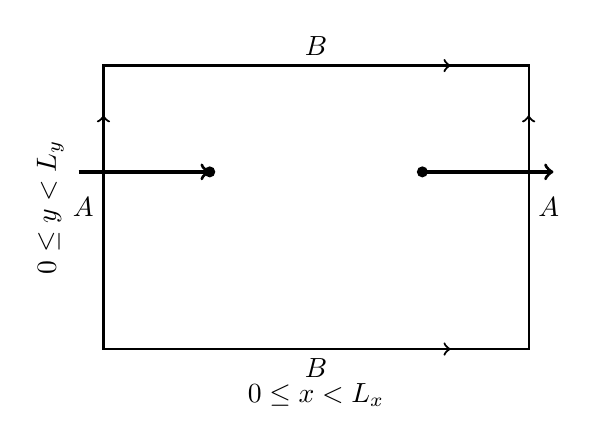
\begin{tikzpicture}[x=0.9cm,y=0.9cm]
\draw[thick] (0,0) rectangle (6,4);
\draw[->,thick] (0,0.7) -- (0,3.3);
\draw[->,thick] (6,0.7) -- (6,3.3);
\draw[->,thick] (1.1,0) -- (4.9,0);
\draw[->,thick] (1.1,4) -- (4.9,4);
\node[left] at (0,2) {$A$};
\node[right] at (6,2) {$A$};
\node[below] at (3,0) {$B$};
\node[above] at (3,4) {$B$};
\draw[->,very thick] (4.5,2.5) -- (6.35,2.5);
\draw[->,very thick] (-0.35,2.5) -- (1.5,2.5);
\fill (4.5,2.5) circle (2pt);
\fill (1.5,2.5) circle (2pt);
\node at (3,-0.65) {$0\leq x<L_x$};
\node[rotate=90] at (-0.75,2) {$0\leq y<L_y$};
\end{tikzpicture}
\caption{二維週期空間：標記相同的邊彼此識別，因此粒子穿過一條邊後，會從對邊的對應位置重新出現。}
\end{figure}

\begin{classroomqa}
\lecturetimestamp{01:50:58}
\audiencequestion{週期性構造描述的是空間，還是空間中的物體？}
\lecturerresponse{它描述的是空間。物體和場存在於這個空間中，並遵守其中的識別關係。引入週期性是為了處理無限體積問題；將體積取為很大，並以積分取代動量總和，就能移除週期性。}
\end{classroomqa}

三維的類比是一個立方體，三對相對的面彼此識別：左面與右面相同，上面與下面相同，前面與後面相同。粒子穿過任何一面後，都會從與之識別的另一面重新出現。\footnote{週期立方體及其三對彼此識別的面，見01:51:27--01:52:17。\(k_i\)的顯示公式是將先前條件\(kL=2\pi n\)分別寫成各分量的形式，並套用於三個週期方向。}三個動量分量滿足
\begin{equation}
k_i=\frac{2\pi n_i}{L_i},
\qquad i=x,y,z,
\end{equation}
每個方向各有一個整數\(n_i\)。依照相同規則，可以定義任意維度的環面。

\begin{figure}[t]
\centering
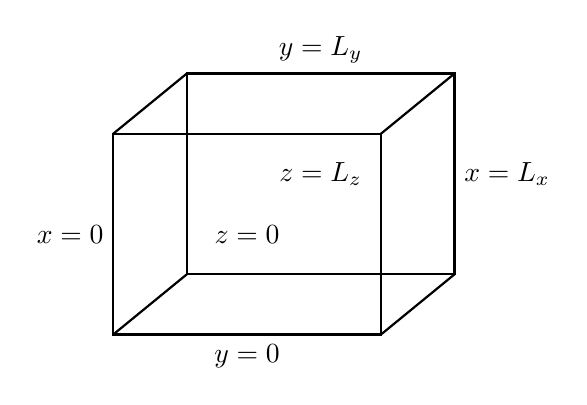
\begin{tikzpicture}[scale=0.85]
\draw[thick] (0,0) rectangle (4,3);
\draw[thick] (1.1,0.9) rectangle (5.1,3.9);
\draw[thick] (0,0) -- (1.1,0.9);
\draw[thick] (4,0) -- (5.1,0.9);
\draw[thick] (4,3) -- (5.1,3.9);
\draw[thick] (0,3) -- (1.1,3.9);
\node[left] at (0,1.5) {$x=0$};
\node[right] at (5.1,2.4) {$x=L_x$};
\node[below] at (2,0) {$y=0$};
\node[above] at (3.1,3.9) {$y=L_y$};
\node at (2,1.5) {$z=0$};
\node at (3.1,2.4) {$z=L_z$};
\end{tikzpicture}
\caption{三維週期空間可表示為立方體，並將每對相對的面彼此識別。}
\end{figure}

\begin{classroomqa}
\lecturetimestamp{01:52:20}
\audiencequestion{場論會為空間選定一個實際的網格大小嗎？}
\lecturerresponse{這是個推測性的問題。就此處的實際用途而言，空間是連續的。量子是粒子，而不是空間網格的格點。在圓周構造中，變成離散的是動量；位置仍是連續且具有週期性。}
\end{classroomqa}

\editorialnote{關於網格大小的問答中有一段很長的文字受損，雖提及普朗克尺度，卻無法還原出任何關於空間是否具有基本離散性的主張。此處不據此推論。}

\(k\)的離散性完全是施加週期波函數的結果，並不能證明座標\(x\)本身位於格點上。探討空間是否可能具有基本的微觀結構是合理的，但那是另一個推測性的問題。

\section{費米子與外場}

玻色模態允許任意非負的佔據數。費米子的情形則相反：泡利不相容原理禁止兩個全同費米子佔據同一個狀態。

\begin{classroomqa}
\lecturetimestamp{01:55:13}
\audiencequestion{把對易子換成反對易子，就能得到最簡單的費米子理論嗎？}
\lecturerresponse{基本上是。對易子是\([A,B]=AB-BA\)，反對易子則是\(\{A,B\}=AB+BA\)。相應的費米子產生與湮滅代數實現了泡利不相容原理：不能將第二個全同費米子放入已被佔據的狀態。詳細理論留待後續討論。}
\end{classroomqa}

兩種乘積只差一個符號：
\begin{equation}
[A,B]=AB-BA,
\qquad
\{A,B\}=AB+BA.
\end{equation}
交換算符次序時，對易子會變號，反對易子則不變。若反對易子為零，則
\begin{equation}
\{A,B\}=0
\quad\Longrightarrow\quad
AB=-BA.
\end{equation}
對這樣的一對算符，交換兩個費米子算符的次序會改變符號。這比一般的可交換情形更不尋常；在一般情形中，\([A,B]=0\)會得到\(AB=BA\)。將玻色子的對易關係換成相應的反對易代數，是導入費米子的數學改變；詳細推導留待後續討論。

反對易關係帶來的統計行為，與玻色子的情形相反。全同費米子不會受激而聚集在同一模態；模態一旦被佔據，就會阻止另一個全同費米子進入。單一費米子態最多只能容納一個全同費米子，因此無法靠在同一態中放入任意多個全同費米子來得到經典場極限。

\begin{classroomqa}
\lecturetimestamp{01:58:03}
\audiencequestion{{\proseunicodefont α} 粒子由費米子組成，怎麼會是玻色子？}
\lecturerresponse{由偶數個費米子組成的束縛複合體，可以具有玻色統計。將多個這樣的複合玻色子放入同一個整體狀態，並不等於將它們各自的費米子組分放入同一個全同單粒子態。}
\end{classroomqa}

複合粒子的統計性質，是指束縛物體整體的性質。因此，費米子組分可以結合成表現為玻色子的物體，同時仍不違反組分所遵守的泡利不相容原理。

\begin{classroomqa}
\lecturetimestamp{01:58:33}
\audiencequestion{如何納入外場？}
\lecturerresponse{到目前為止，這個構造尚未納入任何外部背景場。可以將這種場指定為經典場，也可以用含有大量量子的狀態，以量子力學方式表示。}
\end{classroomqa}

要讓這兩種描述相符，大佔據數態必須經過適當準備，並具有相位相干性；只有粒子數大還不夠。\footnote{問答中提到了大量量子所提供的尺度。此處另指出相位相干也是必要條件，以免將大佔據數本身誤認為足以形成經典場。}在這個半經典區域中，兩者的效應除了微小的量子偏差外彼此相符。這是基本的一致性條件：當單一量子的效應不可忽略時，電磁場必須描述離散光子；而含有大量光子且具有適當相位相干性的狀態，則必須重現熟悉的經典電磁波效應。
